\documentclass[aspectratio=169,11pt]{beamer}
\usetheme{metropolis}
\usepackage{tikz}
\usetikzlibrary{arrows.meta,positioning,decorations.pathmorphing,calc,shapes.geometric,decorations.pathreplacing,patterns}
\usepackage{pgfplots}
\pgfplotsset{compat=1.18}
\usepackage{booktabs}
\usepackage{xcolor}
\usepackage{amsmath}
\usepackage{graphicx}
\graphicspath{{figures/}}

\definecolor{evidence}{HTML}{2196F3}
\definecolor{choice}{HTML}{E91E63}
\definecolor{geometry}{HTML}{4CAF50}
\definecolor{causal}{HTML}{FF9800}
\definecolor{neutral}{HTML}{9E9E9E}
\definecolor{pass}{HTML}{4CAF50}
\definecolor{fail}{HTML}{F44336}
\definecolor{partial}{HTML}{FF9800}
\definecolor{dimhigh}{HTML}{D32F2F}
\definecolor{dimlow}{HTML}{1565C0}
\definecolor{bg}{HTML}{FAFAFA}

\title{Geometric Structure in Neural Population Codes}
\subtitle{A tool-comparison framework for causal neural geometry\\[0.3em]
{\small Exploratory results on Steinmetz 2019}}
\author{Elliott Tower}
\date{2026}
\institute{}

\begin{document}

\maketitle

%% ============================================================
%% PART 1: SETUP — accessible framing
%% ============================================================

%% --- SLIDE: The basic question ---
\begin{frame}{The question}

When a population of neurons fires together during a decision, does the \textbf{shape} of that activity matter---or just the individual firing rates?

\vspace{1em}

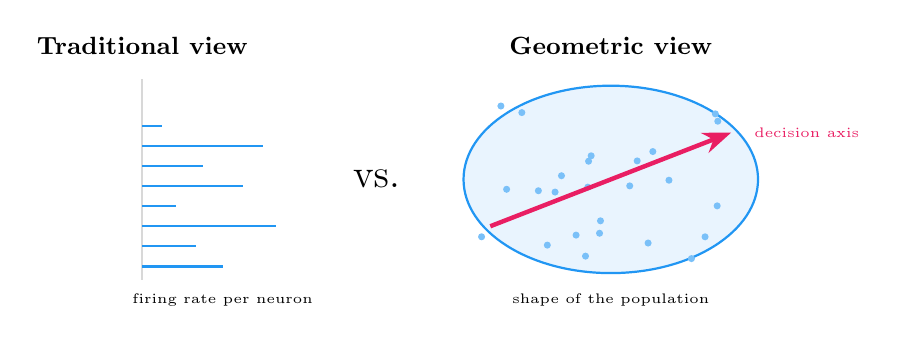
\begin{tikzpicture}[scale=0.85]
  % Left: single neuron view
  \node[font=\small\bfseries] at (0,3.5) {Traditional view};
  \draw[neutral!40,thick] (0,0) -- (0,3);
  \foreach \y/\h in {0.2/1.2, 0.5/0.8, 0.8/2.0, 1.1/0.5, 1.4/1.5, 1.7/0.9, 2.0/1.8, 2.3/0.3} {
    \draw[evidence,thick] (0,\y) -- (\h,\y);
  }
  \node[font=\tiny] at (1.2,-0.3) {firing rate per neuron};

  % Arrow
  \node[font=\Large] at (3.5,1.5) {vs.};

  % Right: population geometry view
  \node[font=\small\bfseries] at (7,3.5) {Geometric view};
  \fill[evidence!10] (7,1.5) ellipse (2.2 and 1.4);
  \draw[evidence,thick] (7,1.5) ellipse (2.2 and 1.4);
  % Points = trials
  \foreach \i in {1,...,25} {
    \pgfmathsetmacro{\rx}{2.0*rand}
    \pgfmathsetmacro{\ry}{1.2*rand}
    \fill[evidence!60] (7+\rx,1.5+\ry) circle (1.5pt);
  }
  \draw[choice,ultra thick,-{Stealth}] (5.2,0.8) -- (8.8,2.2);
  \node[choice,font=\tiny,anchor=west] at (9,2.2) {decision axis};
  \node[font=\tiny] at (7,-0.3) {shape of the population};
\end{tikzpicture}

\vspace{0.5em}
We tested this on real brain recordings, using multiple tools, with causal interventions and validity checks.
\end{frame}

%% --- SLIDE: What is neural geometry? ---
\begin{frame}{What is ``neural geometry''?}
\begin{columns}[T]
\begin{column}{0.55\textwidth}
{\small Each \textbf{trial} produces a pattern of activity across a collection of neurons. Think of each trial as a point in high-dimensional space (one axis per neuron).}

\vspace{0.3em}
{\small ``Geometry'' = what \textbf{shape} do those points form?}
\begin{itemize}\setlength\itemsep{0pt}
  \item {\small Cluster into groups? (categories)}
  \item {\small Spread along a line? (gradient)}
  \item {\small Form a loop? (periodic variable)}
  \item {\small Lie on a flat sheet or curved surface?}
\end{itemize}

\vspace{0.3em}
{\small The shape constrains what information the brain can extract downstream.}
\end{column}
\begin{column}{0.42\textwidth}
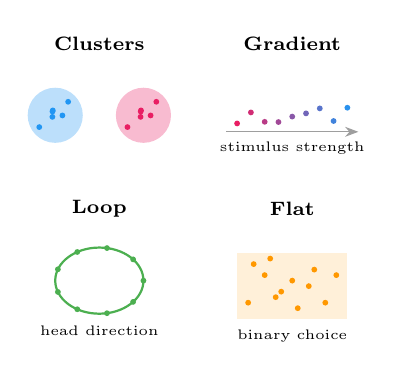
\begin{tikzpicture}[scale=0.7]
  % Example 1: clusters
  \node[font=\scriptsize\bfseries] at (0,5.0) {Clusters};
  \fill[evidence!30] (-0.8,3.7) circle (0.5);
  \fill[choice!30] (0.8,3.7) circle (0.5);
  \foreach \i in {1,...,6} {
    \pgfmathsetmacro{\rx}{0.3*rand}
    \pgfmathsetmacro{\ry}{0.3*rand}
    \fill[evidence] (-0.8+\rx,3.7+\ry) circle (1.5pt);
    \fill[choice] (0.8+\rx,3.7+\ry) circle (1.5pt);
  }

  % Example 2: line/gradient
  \node[font=\scriptsize\bfseries] at (3.5,5.0) {Gradient};
  \foreach \i in {0,...,8} {
    \pgfmathsetmacro{\x}{2.5+\i*0.25}
    \pgfmathsetmacro{\c}{\i*12}
    \fill[evidence!\c!choice] (\x,3.7+0.15*rand) circle (1.5pt);
  }
  \draw[neutral,thin,-{Stealth}] (2.3,3.4) -- (4.7,3.4);
  \node[font=\tiny] at (3.5,3.1) {stimulus strength};

  % Example 3: loop
  \node[font=\scriptsize\bfseries] at (0,2.0) {Loop};
  \draw[geometry,thick] (0,0.7) ellipse (0.8 and 0.6);
  \foreach \a in {0,40,...,320} {
    \fill[geometry] ({0.8*cos(\a)},{0.7+0.6*sin(\a)}) circle (1.5pt);
  }
  \node[font=\tiny] at (0,-0.2) {head direction};

  % Example 4: flat sheet
  \node[font=\scriptsize\bfseries] at (3.5,2.0) {Flat};
  \fill[causal!15] (2.5,0) -- (4.5,0) -- (4.5,1.2) -- (2.5,1.2) -- cycle;
  \foreach \rx/\ry in {2.7/0.3, 3.0/0.8, 3.3/0.5, 3.6/0.2, 3.9/0.9,
                       2.8/1.0, 3.2/0.4, 3.5/0.7, 3.8/0.6, 4.1/0.3,
                       3.1/1.1, 4.3/0.8} {
    \fill[causal] (\rx,\ry) circle (1.5pt);
  }
  \node[font=\tiny] at (3.5,-0.3) {binary choice};
\end{tikzpicture}
\end{column}
\end{columns}
\end{frame}

%% --- SLIDE: Two tools for measuring geometry ---
\begin{frame}{Two tools for measuring geometry}
\begin{columns}[T]
\begin{column}{0.48\textwidth}
\centering
\textbf{\textcolor{dimlow}{CKA (linear)}}

\vspace{0.2em}
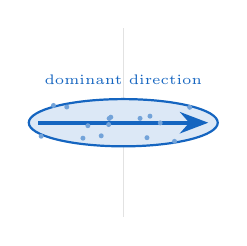
\begin{tikzpicture}[scale=0.6]
  \draw[neutral!30] (-2,0) -- (2,0);
  \draw[neutral!30] (0,-2) -- (0,2);
  \fill[dimlow!15] (0,0) ellipse (2 and 0.5);
  \draw[dimlow,thick] (0,0) ellipse (2 and 0.5);
  \draw[dimlow,ultra thick,-{Stealth}] (-1.8,0) -- (1.8,0);
  \node[dimlow,font=\tiny,above] at (0,0.6) {dominant direction};
  \foreach \i in {1,...,15} {
    \pgfmathsetmacro{\x}{1.8*rand}
    \pgfmathsetmacro{\y}{0.4*rand}
    \fill[dimlow!60] (\x,\y) circle (1.5pt);
  }
\end{tikzpicture}

\vspace{0.2em}
{\small Compares the \textbf{main axis} of variation.}

{\small ``Do the data stretch the same way?''}

{\small Best for low-dimensional data.}
\end{column}
\begin{column}{0.48\textwidth}
\centering
\textbf{\textcolor{dimhigh}{Procrustes (manifold)}}

\vspace{0.2em}
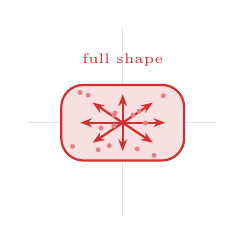
\begin{tikzpicture}[scale=0.6]
  \draw[neutral!30] (-2,0) -- (2,0);
  \draw[neutral!30] (0,-2) -- (0,2);
  \fill[dimhigh!15,rounded corners=8pt] (-1.3,-0.8) rectangle (1.3,0.8);
  \draw[dimhigh,thick,rounded corners=8pt] (-1.3,-0.8) rectangle (1.3,0.8);
  \foreach \a in {0,45,...,315} {
    \draw[dimhigh,thick,-{Stealth[length=1.5mm]}] (0,0) -- ({0.9*cos(\a)},{0.6*sin(\a)});
  }
  \node[dimhigh,font=\tiny,above] at (0,1.0) {full shape};
  \foreach \i in {1,...,15} {
    \pgfmathsetmacro{\x}{1.1*rand}
    \pgfmathsetmacro{\y}{0.7*rand}
    \fill[dimhigh!60] (\x,\y) circle (1.5pt);
  }
\end{tikzpicture}

\vspace{0.2em}
{\small Compares the \textbf{full shape} via rotation + scaling.}

{\small ``Do the data form the same cloud?''}

{\small Best for high-dimensional data.}
\end{column}
\end{columns}

\vspace{0.3em}
\centering
{\small Most prior work treats these as interchangeable. \textbf{They are not.}}
\end{frame}

%% --- SLIDE: The data ---
\begin{frame}{The data: Steinmetz et al.\ 2019}
\begin{columns}[T]
\begin{column}{0.5\textwidth}
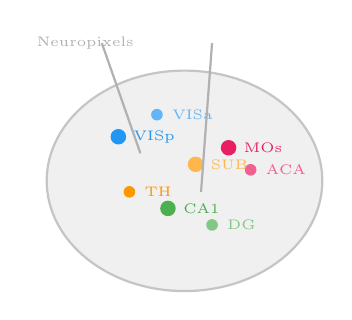
\begin{tikzpicture}[scale=0.7]
  \fill[neutral!15] (0,0) ellipse (2.5 and 2);
  \draw[neutral!60,thick] (0,0) ellipse (2.5 and 2);
  \fill[evidence] (-1.2,0.8) circle (4pt) node[right,font=\tiny,xshift=2pt] {VISp};
  \fill[evidence!70] (-0.5,1.2) circle (3pt) node[right,font=\tiny,xshift=2pt] {VISa};
  \fill[choice] (0.8,0.6) circle (4pt) node[right,font=\tiny,xshift=2pt] {MOs};
  \fill[choice!70] (1.2,0.2) circle (3pt) node[right,font=\tiny,xshift=2pt] {ACA};
  \fill[geometry] (-0.3,-0.5) circle (4pt) node[right,font=\tiny,xshift=2pt] {CA1};
  \fill[geometry!70] (0.5,-0.8) circle (3pt) node[right,font=\tiny,xshift=2pt] {DG};
  \fill[causal] (-1.0,-0.2) circle (3pt) node[right,font=\tiny,xshift=2pt] {TH};
  \fill[causal!70] (0.2,0.3) circle (4pt) node[right,font=\tiny,xshift=2pt] {SUB};
  \draw[neutral!80,thick] (-1.5,2.5) -- (-0.8,0.5);
  \draw[neutral!80,thick] (0.5,2.5) -- (0.3,-0.2);
  \node[font=\tiny,neutral!80] at (-1.8,2.5) {Neuropixels};
\end{tikzpicture}
\end{column}
\begin{column}{0.5\textwidth}
\begin{itemize}
  \item \textbf{39 sessions} from \textbf{10 mice}
  \item \textbf{73 brain regions} recorded simultaneously
  \item Neuropixels probes (${\sim}30{,}000$ neurons total; ${\sim}50$--$500$ per region per session)
  \item \textbf{Task:} visual discrimination \\
    {\small Two screens show visual noise at different contrasts. Mouse turns a wheel toward the higher-contrast side.}
  \item 1,316 pairwise region comparisons
\end{itemize}
\vspace{0.5em}
{\small \textcolor{neutral}{Steinmetz et al., Nature 2019}}
\end{column}
\end{columns}
\end{frame}

%% --- SLIDE: Roadmap ---
\begin{frame}{What we'll cover}
\begin{columns}[T]
\begin{column}{0.48\textwidth}
\textbf{1. Descriptive geometry}\\[0.2em]
{\small Different tools give opposite answers about which brain regions are ``similar.'' We find out why: dimensionality determines which metric you can trust.}

\vspace{0.6em}
\textbf{2. Causal interventions}\\[0.2em]
{\small We borrow a technique from AI interpretability to test whether the geometric structure actually matters for the mouse's decision --- or just looks pretty.}
\end{column}
\begin{column}{0.48\textwidth}
\textbf{3. Beyond linear subspaces}\\[0.2em]
{\small LDA is linear and correlational. A structured VAE finds subspaces that are 3.4$\times$ more causally effective --- the true signal was there, we were using the wrong tool.}

\vspace{0.6em}
\textbf{4. Validation \& what it means}\\[0.2em]
{\small Eight tests designed to catch us if we're fooling ourselves. Novel predictions, honest limitations, and the punchline.}
\end{column}
\end{columns}
\end{frame}

%% --- SLIDE: Intellectual grounding ---
\begin{frame}{Intellectual grounding}
\begin{itemize}\setlength\itemsep{3pt}
  \item {\small \textbf{Structured representation learning} (Esmaeili et al.\ 2019; Opper et al.\ 2023; ICML 2025)---structural priors improve identifiability. Our metric taxonomy is an inductive bias argument.}
  \item {\small \textbf{Relational causal models} (Maier et al.\ 2013; Arbour et al.\ 2016)---brain regions interact as a network, not i.i.d.\ samples. Causal tools need adaptation.}
  \item {\small \textbf{Dynamical systems} (Sussillo \& Barak 2013; Vyas et al.\ 2020)---network dynamics and computational capacity. Our rotation findings connect here.}
\end{itemize}

\vspace{0.3em}
{\small Validity framework from philosophy of science (Mayo 2018, Craver 2007, Shallice 1988) and causal inference (Pearl \& Bareinboim 2011, Woodward 2003).}
\end{frame}

%% ============================================================
%% PART 2: FINDINGS — descriptive geometry
%% ============================================================
\section{What we found: the tools disagree}

%% --- SLIDE: Why they disagree — concrete example ---
\begin{frame}{Why CKA and Procrustes give opposite answers}
\begin{columns}[T]
\begin{column}{0.5\textwidth}
\centering
\textbf{\textcolor{dimlow}{Low-dimensional region (VISp-type)}}

\vspace{0.3em}
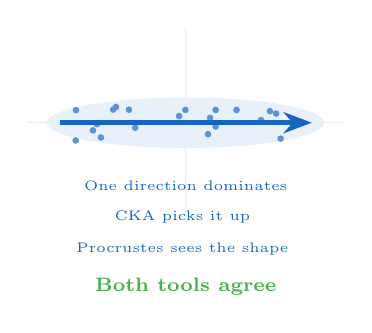
\begin{tikzpicture}[scale=0.8]
  \draw[neutral!20] (-2.5,0) -- (2.5,0);
  \draw[neutral!20] (0,-1.5) -- (0,1.5);

  % Elongated cloud along one axis
  \fill[dimlow!10] (0,0) ellipse (2.2 and 0.4);
  \foreach \i in {1,...,20} {
    \pgfmathsetmacro{\x}{2.0*rand}
    \pgfmathsetmacro{\y}{0.3*rand}
    \fill[dimlow!70] (\x,\y) circle (1.5pt);
  }
  \draw[dimlow,ultra thick,-{Stealth}] (-2,0) -- (2,0);

  \node[font=\tiny,dimlow,align=center] at (0,-1.0) {One direction dominates};
  \node[font=\tiny,dimlow,align=center] at (0,-1.5) {CKA picks it up $\checkmark$};
  \node[font=\tiny,dimlow,align=center] at (0,-2.0) {Procrustes sees the shape $\checkmark$};
  \node[font=\scriptsize,pass] at (0,-2.6) {\textbf{Both tools agree}};
\end{tikzpicture}
\end{column}
\begin{column}{0.5\textwidth}
\centering
\textbf{\textcolor{dimhigh}{High-dimensional region (MOs-type)}}

\vspace{0.3em}
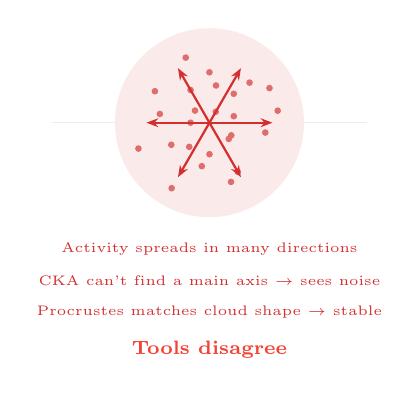
\begin{tikzpicture}[scale=0.8]
  \draw[neutral!20] (-2.5,0) -- (2.5,0);
  \draw[neutral!20] (0,-1.5) -- (0,1.5);

  % Spherical cloud — no dominant axis
  \fill[dimhigh!10] (0,0) circle (1.5);
  \foreach \a/\r in {15/0.4, 45/0.9, 80/0.6, 110/1.1, 140/0.3,
                      170/0.8, 200/1.2, 230/0.5, 260/0.7, 290/1.0,
                      320/0.4, 350/0.9, 30/1.1, 60/0.2, 90/0.8,
                      120/0.6, 150/1.0, 180/0.3, 210/0.7, 240/1.2,
                      270/0.5, 300/0.9, 330/0.4, 10/1.1, 50/0.6} {
    \fill[dimhigh!70] ({(\r)*cos(\a)},{(\r)*sin(\a)}) circle (1.5pt);
  }
  % Multiple equal arrows
  \foreach \a in {0,60,...,300} {
    \draw[dimhigh,thick,-{Stealth[length=1.5mm]}] (0,0) -- ({1.0*cos(\a)},{1.0*sin(\a)});
  }

  \node[font=\tiny,dimhigh,align=center] at (0,-2.0) {Activity spreads in many directions};
  \node[font=\tiny,dimhigh,align=center] at (0,-2.5) {CKA can't find a main axis $\to$ sees noise};
  \node[font=\tiny,dimhigh,align=center] at (0,-3.0) {Procrustes matches cloud shape $\to$ stable};
  \node[font=\scriptsize,fail] at (0,-3.6) {\textbf{Tools disagree}};
\end{tikzpicture}
\end{column}
\end{columns}
\end{frame}

%% --- SLIDE: The anti-correlation — data ---
\begin{frame}{The data: CKA and Procrustes are anti-correlated}
\begin{columns}[T]
\begin{column}{0.68\textwidth}
\centering
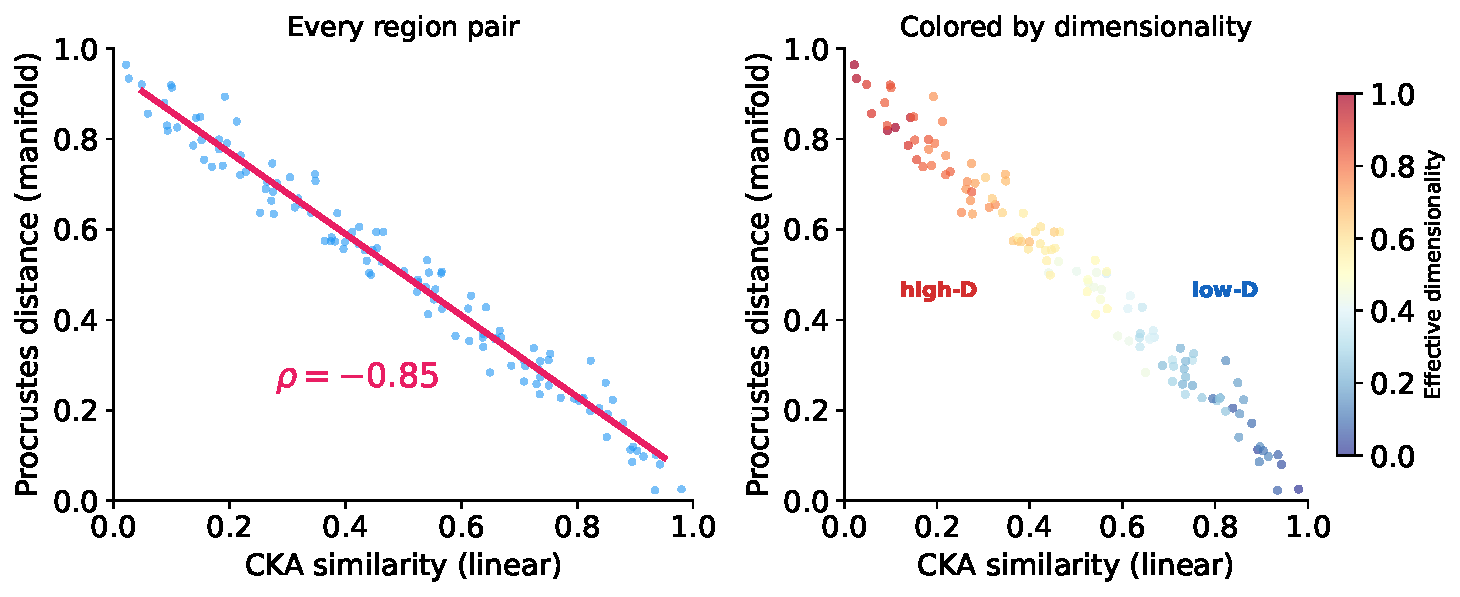
\includegraphics[width=\linewidth]{anticorrelation_scatter.pdf}
\end{column}
\begin{column}{0.30\textwidth}
\vspace{0.5em}
{\small Each dot is a pair of brain regions. The two tools rank them in \textbf{opposite order} (correlation $= -0.85$; $-1$ would be perfect reversal).}

\vspace{0.5em}
{\small \textbf{Why?} The right panel colors dots by how ``spread out'' the neural activity is. Blue dots (compact activity) make both tools agree. Red dots (diffuse activity) make them disagree.}

\vspace{0.2em}
{\small Accounting for spread, disagreement shrinks from $-0.85$ to $-0.31$. Found in 5 sessions, confirmed across all 39. \textbf{Takeaway:} the tool you pick determines what you find.}
\end{column}
\end{columns}
\end{frame}

%% --- SLIDE: Eigenvalue spectra ---
\begin{frame}{What determines dimensionality?}
\centering
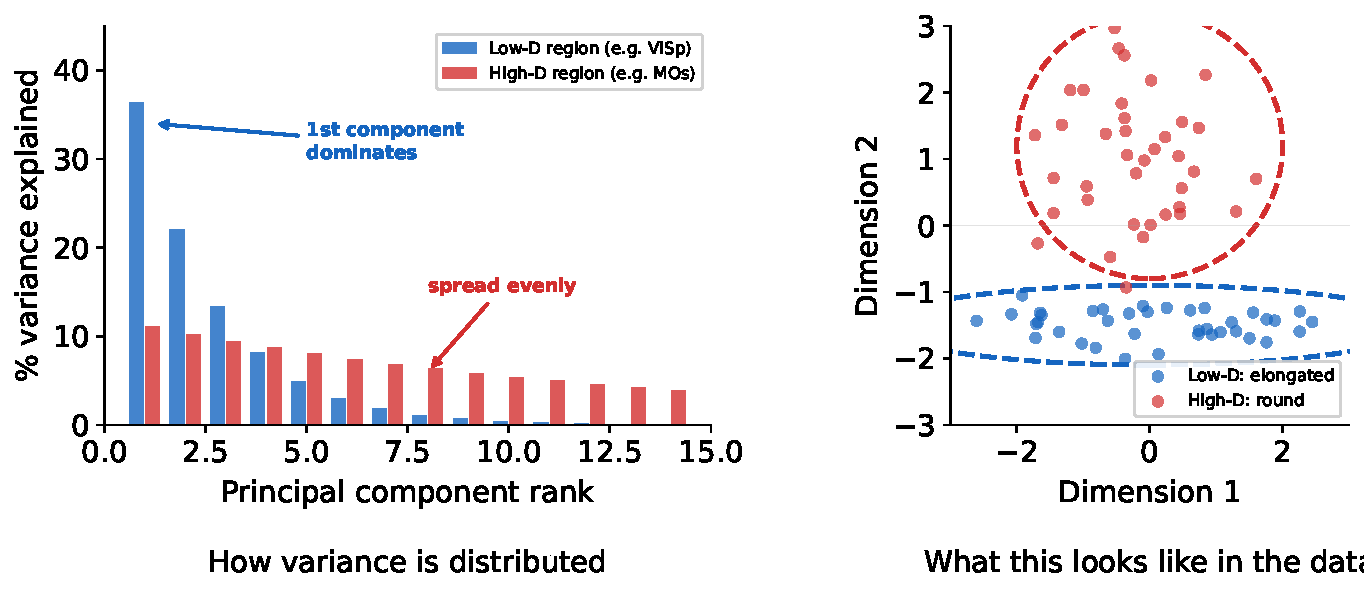
\includegraphics[width=0.85\linewidth]{eigenvalue_spectra.pdf}

\vspace{0.5em}
{\small Across all 73 regions, the \textbf{shape} of how variance falls off is nearly identical (correlation $0.94$ out of $1.0$). But \textbf{which neurons} carry the variance is completely different per region (correlation $0.09$, barely above zero). Same scaffolding, different content.}
\end{frame}

%% ============================================================
%% PART 3: MORE DESCRIPTIVE FINDINGS
%% ============================================================

%% --- SLIDE: Rotation ---
\begin{frame}{Every brain region rotates (but at very different speeds)}
\begin{columns}[T]
\begin{column}{0.42\textwidth}
\centering
{\small \textbf{What rotation means}}

\vspace{0.3em}
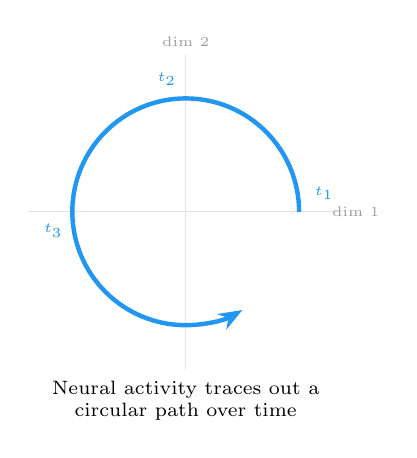
\begin{tikzpicture}[scale=0.8]
  \draw[neutral!30,thin] (-2.5,0) -- (2.5,0);
  \draw[neutral!30,thin] (0,-2.5) -- (0,2.5);
  \node[font=\tiny,neutral] at (2.7,0) {dim 1};
  \node[font=\tiny,neutral] at (0,2.7) {dim 2};
  \draw[evidence,ultra thick,-{Stealth[length=3mm]}]
    (1.8,0) arc[start angle=0, end angle=300, radius=1.8];
  \node[font=\tiny,evidence] at (2.2,0.3) {$t_1$};
  \node[font=\tiny,evidence] at (-0.3,2.1) {$t_2$};
  \node[font=\tiny,evidence] at (-2.1,-0.3) {$t_3$};
  \node[font=\scriptsize,align=center] at (0,-3) {Neural activity traces out a\\circular path over time};
\end{tikzpicture}
\end{column}
\begin{column}{0.56\textwidth}
\centering
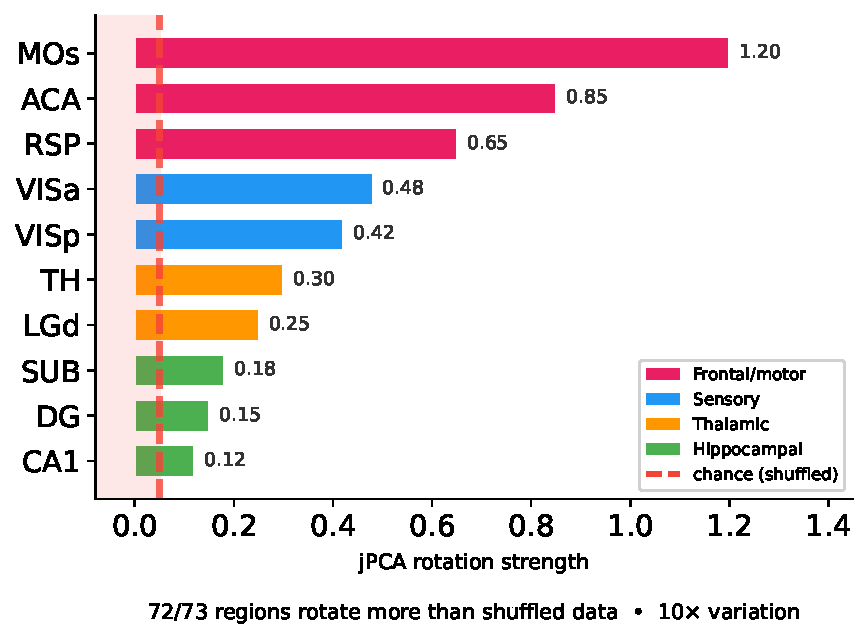
\includegraphics[width=\linewidth]{jpca_rotation.pdf}
\end{column}
\end{columns}
\end{frame}

%% --- SLIDE: Anatomy recovery (sanity check) ---
\begin{frame}{Sanity check: geometry tracks known anatomy}
\begin{columns}[T]
\begin{column}{0.5\textwidth}
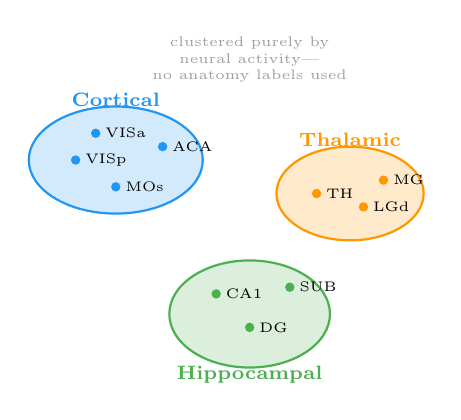
\begin{tikzpicture}[scale=0.85]
  \fill[evidence!20] (-1.5,2) ellipse (1.3 and 0.8);
  \draw[evidence,thick] (-1.5,2) ellipse (1.3 and 0.8);
  \node[evidence,font=\scriptsize\bfseries] at (-1.5,2.9) {Cortical};
  \foreach \name/\x/\y in {VISp/-2.1/2, MOs/-1.5/1.6, ACA/-0.8/2.2, VISa/-1.8/2.4} {
    \fill[evidence] (\x,\y) circle (2pt);
    \node[font=\tiny,right] at (\x,\y) {\name};
  }
  \fill[causal!20] (2,1.5) ellipse (1.1 and 0.7);
  \draw[causal,thick] (2,1.5) ellipse (1.1 and 0.7);
  \node[causal,font=\scriptsize\bfseries] at (2,2.3) {Thalamic};
  \foreach \name/\x/\y in {TH/1.5/1.5, LGd/2.2/1.3, MG/2.5/1.7} {
    \fill[causal] (\x,\y) circle (2pt);
    \node[font=\tiny,right] at (\x,\y) {\name};
  }
  \fill[geometry!20] (0.5,-0.3) ellipse (1.2 and 0.8);
  \draw[geometry,thick] (0.5,-0.3) ellipse (1.2 and 0.8);
  \node[geometry,font=\scriptsize\bfseries] at (0.5,-1.2) {Hippocampal};
  \foreach \name/\x/\y in {CA1/0/0, DG/0.5/-0.5, SUB/1.1/0.1} {
    \fill[geometry] (\x,\y) circle (2pt);
    \node[font=\tiny,right] at (\x,\y) {\name};
  }
  \node[font=\tiny,neutral,align=center] at (0.5,3.5) {clustered purely by\\neural activity---\\no anatomy labels used};
\end{tikzpicture}
\end{column}
\begin{column}{0.48\textwidth}
{\small We grouped brain regions \emph{purely by how similar their neural activity looks}---no anatomy labels as input.}

\vspace{0.3em}
{\small \textbf{Result:} the algorithm found three groups matching the textbook cortical / thalamic / hippocampal division on its own.}

\vspace{0.3em}
{\small \textbf{Why this matters:} CKA is a general-purpose metric, not designed for neuroscience. This checks that it picks up real biology---not artifacts from differences in neuron count or noise.}

\vspace{0.3em}
{\small Same result within individual sessions and across animals.}
\end{column}
\end{columns}
\end{frame}

%% ============================================================
%% PART 4: CAUSAL INTERVENTIONS
%% ============================================================
\section{Is the geometry causal?}

%% --- SLIDE: From correlation to causation ---
\begin{frame}{From observation to intervention}
\begin{columns}[T]
\begin{column}{0.48\textwidth}
\centering
{\small \textbf{So far:} observation only}
\vspace{0.3em}

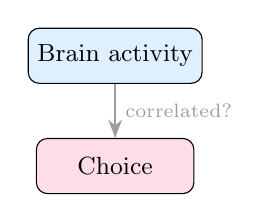
\begin{tikzpicture}[scale=0.7]
  \node[draw,rounded corners,fill=evidence!15,minimum width=2cm,minimum height=0.7cm,font=\small] (brain) at (0,2) {Brain activity};
  \node[draw,rounded corners,fill=choice!15,minimum width=2cm,minimum height=0.7cm,font=\small] (choice) at (0,0) {Choice};
  \draw[-{Stealth},thick,neutral] (brain) -- node[right,font=\scriptsize] {correlated?} (choice);
\end{tikzpicture}

\vspace{0.5em}
{\small We measured shapes and distances.\\ But correlation $\neq$ causation.}

\vspace{0.5em}
{\small Maybe neurons that ``look important'' by CKA don't actually \emph{do} anything for the decision.}
\end{column}
\begin{column}{0.48\textwidth}
\centering
{\small \textbf{Now:} intervention}
\vspace{0.3em}

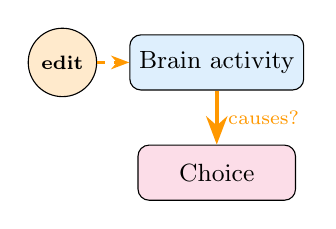
\begin{tikzpicture}[scale=0.7]
  \node[draw,rounded corners,fill=evidence!15,minimum width=2cm,minimum height=0.7cm,font=\small] (brain2) at (0,2) {Brain activity};
  \node[draw,rounded corners,fill=choice!15,minimum width=2cm,minimum height=0.7cm,font=\small] (choice2) at (0,0) {Choice};
  \draw[-{Stealth},ultra thick,causal] (brain2) -- node[right,font=\scriptsize,causal] {causes?} (choice2);

  % Intervention arrow
  \node[draw,circle,fill=causal!20,minimum size=0.7cm,font=\scriptsize\bfseries] (do) at (-2.8,2) {edit};
  \draw[-{Stealth},thick,causal,dashed] (do) -- (brain2);
\end{tikzpicture}

\vspace{0.5em}
{\small We \textbf{change} specific dimensions of the neural activity and check if a trained classifier's prediction changes.}

\vspace{0.5em}
{\small If editing a subspace flips the classifier's output, that subspace causally mediates our \emph{estimate} of the decision---not the mouse's actual choice, which we can't re-run.}
\end{column}
\end{columns}
\end{frame}

%% --- SLIDE: Where this idea comes from ---
\begin{frame}{Inspiration: how AI researchers test neural networks}
\begin{columns}[T]
\begin{column}{0.55\textwidth}
{\small In AI safety research (\textbf{mechanistic interpretability}), scientists test neural networks by:}

\begin{enumerate}\setlength\itemsep{0pt}
  \item {\small Run a model on two different inputs}
  \item {\small Find the internal representation}
  \item {\small \textbf{Swap} part of one into the other}
  \item {\small Check if the output changes}
\end{enumerate}

\vspace{0.1em}
{\small This is \textbf{interchange intervention analysis} (Geiger et al.\ 2024). The same logic works for biological neurons: language model $\to$ mouse brain, text $\to$ visual stimuli.}

\vspace{0.2em}
{\scriptsize \textbf{Our contribution:} neuroscience targets \emph{neurons} (optogenetics); AI targets \emph{subspaces} (in silico). We bring subspace-level interventions to biological recordings.}
\end{column}
\begin{column}{0.42\textwidth}
\centering
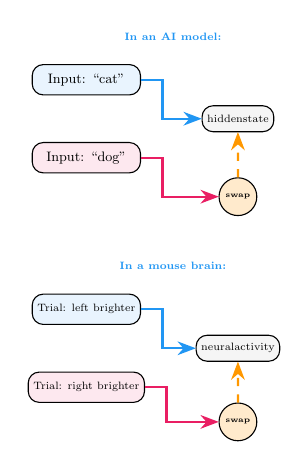
\begin{tikzpicture}[scale=0.55, every node/.style={transform shape},
  box/.style={draw,rounded corners,minimum width=2.5cm,minimum height=0.7cm,font=\small},
]
  % AI version
  \node[font=\scriptsize\bfseries,evidence] at (2,5) {In an AI model:};
  \node[box,fill=evidence!10] (in1) at (0,4) {Input: ``cat''};
  \node[box,fill=choice!10] (in2) at (0,2.2) {Input: ``dog''};
  \node[draw,rounded corners,fill=neutral!10,minimum width=1.5cm,minimum height=0.6cm,font=\scriptsize] (hidden) at (3.5,3.1) {hidden\\state};
  \node[draw,circle,fill=causal!20,minimum size=0.7cm,font=\tiny\bfseries] (sw) at (3.5,1.3) {swap};

  \draw[-{Stealth},thick,evidence] (in1.east) -- ++(0.5,0) |- (hidden);
  \draw[-{Stealth},thick,choice] (in2.east) -- ++(0.5,0) |- (sw);
  \draw[-{Stealth},thick,causal,dashed] (sw) -- (hidden);

  % Brain version
  \node[font=\scriptsize\bfseries,evidence] at (2,-0.3) {In a mouse brain:};
  \node[box,fill=evidence!10,font=\scriptsize] (t1) at (0,-1.3) {Trial: left brighter};
  \node[box,fill=choice!10,font=\scriptsize] (t2) at (0,-3.1) {Trial: right brighter};
  \node[draw,rounded corners,fill=neutral!10,minimum width=1.5cm,minimum height=0.6cm,font=\scriptsize] (neur) at (3.5,-2.2) {neural\\activity};
  \node[draw,circle,fill=causal!20,minimum size=0.7cm,font=\tiny\bfseries] (sw2) at (3.5,-3.9) {swap};

  \draw[-{Stealth},thick,evidence] (t1.east) -- ++(0.5,0) |- (neur);
  \draw[-{Stealth},thick,choice] (t2.east) -- ++(0.5,0) |- (sw2);
  \draw[-{Stealth},thick,causal,dashed] (sw2) -- (neur);
\end{tikzpicture}
\end{column}
\end{columns}
\end{frame}

%% --- SLIDE: What "swapping" means concretely ---
\begin{frame}{What ``swapping a subspace'' means}
\begin{columns}[T]
\begin{column}{0.55\textwidth}
{\small Neural activity in a brain region is a \textbf{high-dimensional vector}---each neuron is one dimension. (E.g., 200 neurons = 200 dimensions.)}

\vspace{0.3em}
{\small Not all dimensions matter equally. We hypothesize that a \textbf{small subset of directions} (a ``subspace'') encodes the evidence signal.}

\vspace{0.3em}
{\small \textbf{The swap:}}
\begin{enumerate}\setlength\itemsep{2pt}
  \item {\small Take two trials with opposite evidence}
  \item {\small Swap \textbf{only} what we think is the evidence-related part between them}
  \item {\small Leave everything else unchanged}
  \item {\small Check: does the output flip?}
\end{enumerate}

\vspace{0.3em}
{\small Same logic in both: swap part of the internal state, check if the output changes.}
\end{column}
\begin{column}{0.42\textwidth}
\centering
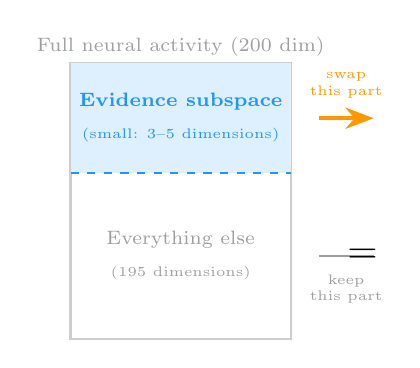
\begin{tikzpicture}[scale=0.7]
  % Full space
  \draw[thick,neutral!50] (0,0) rectangle (4,5);
  \node[font=\scriptsize,neutral] at (2,5.3) {Full neural activity (200 dim)};

  % Evidence subspace highlight
  \fill[evidence!15] (0,3) rectangle (4,5);
  \draw[evidence,thick,dashed] (0,3) -- (4,3);
  \node[evidence,font=\scriptsize\bfseries] at (2,4.3) {Evidence subspace};
  \node[evidence,font=\tiny] at (2,3.7) {(small: 3--5 dimensions)};

  % Other dimensions
  \node[neutral,font=\scriptsize] at (2,1.8) {Everything else};
  \node[neutral,font=\tiny] at (2,1.2) {(195 dimensions)};

  % Swap arrows
  \draw[causal,ultra thick,-{Stealth}] (4.5,4) -- (5.5,4);
  \node[causal,font=\tiny,align=center] at (5,4.6) {swap\\this part};

  \draw[neutral,thick] (4.5,1.5) -- (5.5,1.5);
  \node[neutral,font=\tiny,align=center] at (5,0.9) {keep\\this part};
  \node[font=\Large] at (5.3,1.5) {$=$};
\end{tikzpicture}
\end{column}
\end{columns}
\end{frame}

%% --- SLIDE: Recap the task ---
\begin{frame}{Recap: what the mouse is doing}
\begin{columns}[T]
\begin{column}{0.5\textwidth}
\centering
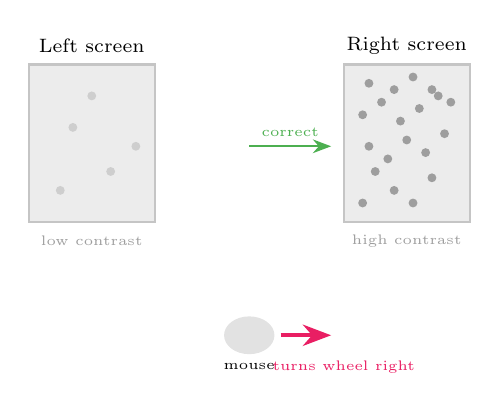
\begin{tikzpicture}[scale=0.8]
  % Left screen
  \fill[neutral!20] (-3.5,0) rectangle (-1.5,2.5);
  \draw[neutral!60,thick] (-3.5,0) rectangle (-1.5,2.5);
  \node[font=\scriptsize] at (-2.5,2.8) {Left screen};
  % Sparse dots = low contrast (fixed positions)
  \fill[neutral!50] (-3.0,0.5) circle (2pt);
  \fill[neutral!50] (-2.8,1.5) circle (2pt);
  \fill[neutral!50] (-2.2,0.8) circle (2pt);
  \fill[neutral!50] (-2.5,2.0) circle (2pt);
  \fill[neutral!50] (-1.8,1.2) circle (2pt);
  \node[font=\tiny,neutral] at (-2.5,-0.3) {low contrast};

  % Right screen
  \fill[neutral!20] (1.5,0) rectangle (3.5,2.5);
  \draw[neutral!60,thick] (1.5,0) rectangle (3.5,2.5);
  \node[font=\scriptsize] at (2.5,2.8) {Right screen};
  % Dense dots = high contrast (fixed positions)
  \foreach \x/\y in {1.8/0.3, 2.0/0.8, 2.3/0.5, 2.6/0.3, 2.9/0.7,
                      1.9/1.2, 2.2/1.0, 2.5/1.3, 2.8/1.1, 3.1/1.4,
                      1.8/1.7, 2.1/1.9, 2.4/1.6, 2.7/1.8, 3.0/2.0,
                      1.9/2.2, 2.3/2.1, 2.6/2.3, 2.9/2.1, 3.2/1.9} {
    \fill[neutral] (\x,\y) circle (2pt);
  }
  \node[font=\tiny,neutral] at (2.5,-0.3) {high contrast};

  % Mouse + wheel
  \fill[neutral!30] (0,-1.8) ellipse (0.4 and 0.3);
  \node[font=\tiny] at (0,-2.3) {mouse};
  \draw[choice,ultra thick,-{Stealth}] (0.5,-1.8) -- (1.3,-1.8);
  \node[choice,font=\tiny] at (1.5,-2.3) {turns wheel right};

  % Arrow showing correct choice
  \draw[pass,thick,-{Stealth}] (0,1.2) -- (1.3,1.2);
  \node[pass,font=\tiny,above] at (0.65,1.2) {correct};
\end{tikzpicture}
\end{column}
\begin{column}{0.48\textwidth}
\vspace{0.5em}
{\small The mouse sees two screens with random visual noise. One side has \textbf{higher contrast} (more visible dots). The mouse turns a wheel toward that side to get a reward.}

\vspace{0.3em}
{\small \textbf{``Evidence''} = which side has higher contrast. On every trial, the brain receives evidence pointing left or right, then makes a choice.}

\vspace{0.3em}
{\small \textbf{The question:} somewhere in the neural activity, there must be a signal carrying this evidence from sensory areas to the decision. We call it the ``evidence subspace.''}
\end{column}
\end{columns}
\end{frame}

%% --- SLIDE: The intervention ---
\begin{frame}{Applying the swap to our mouse data}
\begin{columns}[T]
\begin{column}{0.55\textwidth}
{\small Two trials where the mouse saw opposite evidence:}
\begin{itemize}\setlength\itemsep{2pt}
  \item {\small Trial A: left side brighter $\to$ chose left}
  \item {\small Trial B: right side brighter $\to$ chose right}
\end{itemize}

\vspace{0.3em}
{\small We swap \textbf{only what we think is the evidence-related part} of the neural activity between them. Everything else stays the same.}

\vspace{0.3em}
{\small A classifier now predicts the \emph{opposite} choice $\to$ those dimensions \textbf{causally carry} the evidence.}

\vspace{0.3em}
{\small We do this for every brain region to map where in the brain evidence is causally routed.}
\end{column}
\begin{column}{0.42\textwidth}
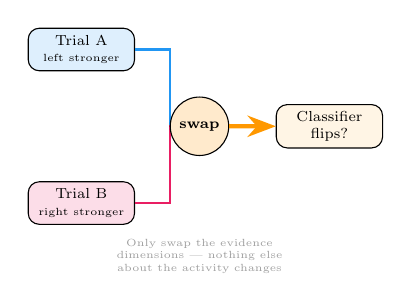
\begin{tikzpicture}[scale=0.75, every node/.style={transform shape},
  box/.style={draw,rounded corners,minimum width=1.8cm,minimum height=0.7cm,font=\scriptsize},
]
  \node[box,fill=evidence!15,align=center] (A) at (0,2.8) {Trial A\\{\tiny left stronger}};
  \node[box,fill=choice!15,align=center] (B) at (0,0.2) {Trial B\\{\tiny right stronger}};

  \draw[evidence,thick,-{Stealth}] (A.east) -- ++(0.6,0) |- (2,1.5);
  \draw[choice,thick,-{Stealth}] (B.east) -- ++(0.6,0) |- (2,1.5);

  \node[draw,circle,fill=causal!20,minimum size=0.9cm,font=\scriptsize\bfseries] (swap) at (2,1.5) {swap};
  \node[box,fill=causal!10,align=center] (out) at (4.2,1.5) {Classifier\\flips?};
  \draw[-{Stealth},ultra thick,causal] (swap) -- (out);

  \node[font=\tiny,neutral,text width=3cm,align=center] at (2,-0.7) {Only swap the evidence\\dimensions --- nothing else\\about the activity changes};
\end{tikzpicture}
\end{column}
\end{columns}
\end{frame}

%% --- SLIDE: Q1 — Why not swap everything? ---
\begin{frame}{Wait --- why not just swap the \emph{entire} recording?}
\begin{columns}[T]
\begin{column}{0.6\textwidth}
{\small \textbf{Good question.} If we replaced \emph{all 200 numbers} from Trial A with Trial B's, the classifier would obviously say ``right.'' We just gave it Trial B's data. That tells us nothing.}

\vspace{0.4em}
{\small \textbf{The power is in swapping only a small part.} We swap \textbf{5 out of 200} dimensions. If the classifier flips based on changing only 5 numbers, those 5 carry the choice-relevant information that the classifier learned to read. The other 195 don't matter \emph{to the classifier}.}

\vspace{0.2em}
{\small \textbf{Caveat:} the classifier is a proxy for the brain's own readout. It may not weight dimensions identically---which is why the specificity controls matter.}

\end{column}
\begin{column}{0.37\textwidth}
\centering
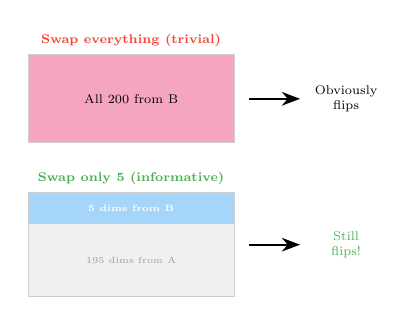
\begin{tikzpicture}[scale=0.65, every node/.style={transform shape}]
  % Full swap = trivial
  \node[font=\scriptsize\bfseries,fail] at (2,5.5) {Swap everything (trivial)};
  \draw[thick,neutral!50] (0,3.5) rectangle (4,5.2);
  \fill[choice!40] (0,3.5) rectangle (4,5.2);
  \node[font=\scriptsize] at (2,4.35) {All 200 from B};
  \draw[-{Stealth},thick] (4.3,4.35) -- (5.3,4.35);
  \node[font=\scriptsize,align=center] at (6.2,4.35) {Obviously\\flips};

  % Partial swap = informative
  \node[font=\scriptsize\bfseries,pass] at (2,2.8) {Swap only 5 (informative)};
  \draw[thick,neutral!50] (0,0.5) rectangle (4,2.5);
  \fill[evidence!40] (0,1.9) rectangle (4,2.5);
  \node[font=\tiny\bfseries,white] at (2,2.2) {5 dims from B};
  \fill[neutral!15] (0,0.5) rectangle (4,1.9);
  \node[neutral,font=\tiny] at (2,1.2) {195 dims from A};
  \draw[-{Stealth},thick] (4.3,1.5) -- (5.3,1.5);
  \node[font=\scriptsize,align=center,pass] at (6.2,1.5) {Still\\flips!};
\end{tikzpicture}
\end{column}
\end{columns}
\end{frame}

%% --- SLIDE: Neural populations encode multiple variables ---
\begin{frame}{Neural populations encode many things at once}
\begin{columns}[T]
\begin{column}{0.55\textwidth}
{\small Prior work shows the same neurons encode multiple variables simultaneously (Steinmetz 2019; Musall 2019; Stringer 2019):}

\vspace{0.2em}
\begin{itemize}\setlength\itemsep{2pt}
  \item {\small \textcolor{evidence}{\textbf{Stimulus evidence}} --- which side brighter}
  \item {\small \textbf{Reaction time} --- how fast the mouse responds}
  \item {\small \textbf{Feedback} --- correct or wrong}
  \item {\small \textbf{Movement} --- wheel, licking, etc.}
\end{itemize}

\vspace{0.2em}
{\small Each occupies a different \textbf{subspace}. We identify them via PCA on the relevant trial labels.}

\vspace{0.2em}
{\small \textbf{Key question:} which subspace actually drives the decision?}
\end{column}
\begin{column}{0.42\textwidth}
\centering
\vspace{0.3em}
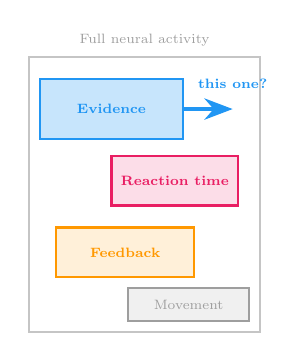
\begin{tikzpicture}[scale=0.7, every node/.style={transform shape}]
  % Full neural space
  \draw[thick,neutral!60] (0,0) rectangle (4.2,5);
  \node[font=\scriptsize,neutral] at (2.1,5.3) {Full neural activity};

  % Subspaces as overlapping rectangles
  \fill[evidence!25] (0.2,3.5) rectangle (2.8,4.6);
  \draw[evidence,thick] (0.2,3.5) rectangle (2.8,4.6);
  \node[evidence,font=\scriptsize\bfseries] at (1.5,4.05) {Evidence};

  \fill[choice!15] (1.5,2.3) rectangle (3.8,3.2);
  \draw[choice,thick] (1.5,2.3) rectangle (3.8,3.2);
  \node[choice,font=\scriptsize\bfseries] at (2.65,2.75) {Reaction time};

  \fill[causal!15] (0.5,1.0) rectangle (3.0,1.9);
  \draw[causal,thick] (0.5,1.0) rectangle (3.0,1.9);
  \node[causal,font=\scriptsize\bfseries] at (1.75,1.45) {Feedback};

  \fill[neutral!15] (1.8,0.2) rectangle (4.0,0.8);
  \draw[neutral,thick] (1.8,0.2) rectangle (4.0,0.8);
  \node[neutral,font=\scriptsize] at (2.9,0.5) {Movement};

  % Arrow to question
  \draw[evidence,ultra thick,-{Stealth}] (2.8,4.05) -- (3.7,4.05);
  \node[evidence,font=\scriptsize\bfseries] at (3.7,4.5) {this one?};
\end{tikzpicture}
\end{column}
\end{columns}
\end{frame}

%% --- SLIDE: Controls — specificity ---
\begin{frame}{How do we know it's \emph{those specific} dimensions?}
\begin{columns}[T]
\begin{column}{0.5\textwidth}
{\small \textbf{We run controls.} Repeat the exact same swap, but targeting different subspaces:}

\vspace{0.1em}
\begin{itemize}\setlength\itemsep{1pt}
  \item {\small \textbf{Reaction time} dims --- barely flips}
  \item {\small \textbf{Feedback} dims --- barely flips}
  \item {\small \textbf{Random} dims --- barely flips}
  \item {\small \textcolor{evidence}{\textbf{Evidence}} dims --- \textbf{yes, it flips}}
\end{itemize}

\vspace{0.2em}
{\small This is \textbf{specificity}: only evidence dimensions produce the effect, not any random 5.}

\vspace{0.2em}
{\small \textbf{Why this matters:} without controls, we'd just be showing \emph{any} 5 dims can disrupt a classifier --- trivial. Specificity is what makes it causal.}
\end{column}
\begin{column}{0.48\textwidth}
\centering
\vspace{-0.3em}
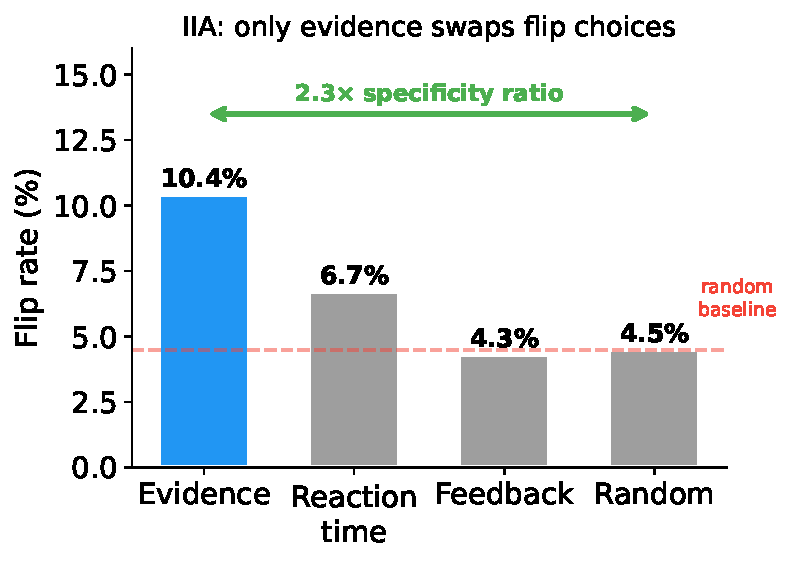
\includegraphics[width=\linewidth]{iia_bars.pdf}
\end{column}
\end{columns}
\end{frame}

%% --- SLIDE: Sufficiency — why it's not circular ---
\begin{frame}{Is this circular?}
\begin{columns}[T]
\begin{column}{0.55\textwidth}
{\small A fair objection: ``you found the subspace with a classifier, then showed the classifier likes it. Of course it does.''}

\vspace{0.5em}
{\small But the subspace and the classifier use \textbf{different information}:}

\vspace{0.3em}
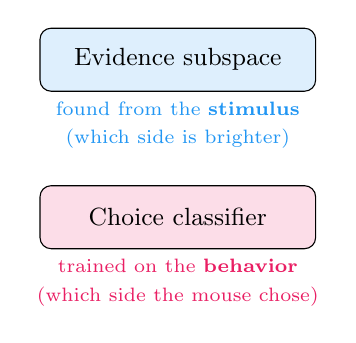
\begin{tikzpicture}[
  box/.style={draw,rounded corners,minimum width=3.5cm,minimum height=0.8cm,font=\small,align=center},
]
  \node[box,fill=evidence!15] (sub) at (0,2) {Evidence subspace};
  \node[font=\scriptsize,evidence,below=0pt of sub] {found from the \textbf{stimulus}};
  \node[font=\scriptsize,evidence,below=10pt of sub] {(which side is brighter)};

  \node[box,fill=choice!15] (cls) at (0,0) {Choice classifier};
  \node[font=\scriptsize,choice,below=0pt of cls] {trained on the \textbf{behavior}};
  \node[font=\scriptsize,choice,below=10pt of cls] {(which side the mouse chose)};
\end{tikzpicture}

\end{column}
\begin{column}{0.43\textwidth}
\vspace{0.5em}
{\small The stimulus and the behavior are \textbf{correlated but not identical}---the mouse sometimes chooses wrong.}

\vspace{0.5em}
{\small So showing that a \emph{stimulus}-defined subspace improves \emph{choice} prediction is genuinely informative: the stimulus signal is what the brain uses for decisions.}

\vspace{0.5em}
{\small \textbf{Ground truth} = the mouse's actual left/right choice. We know this from the experiment.}
\end{column}
\end{columns}
\end{frame}

%% --- SLIDE: Sufficiency — the result ---
\begin{frame}{The evidence subspace is sufficient (and denoises)}
\begin{columns}[T]
\begin{column}{0.5\textwidth}
\centering
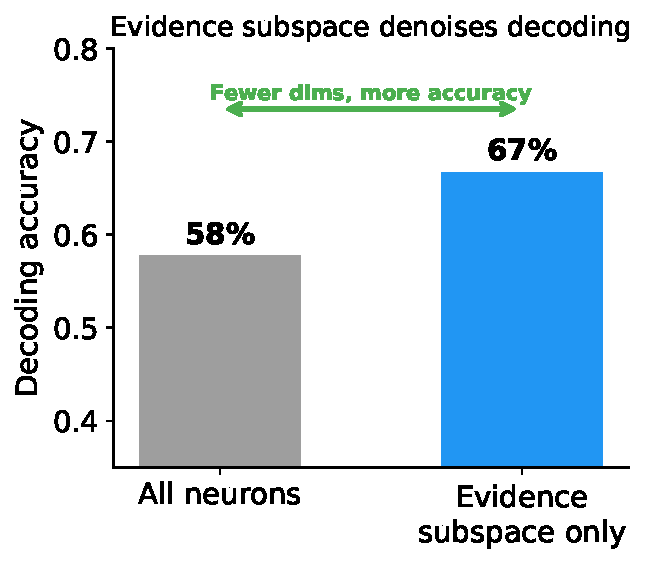
\includegraphics[width=0.85\linewidth]{sufficiency.pdf}
\end{column}
\begin{column}{0.48\textwidth}
Restricting a classifier to \emph{only} the evidence subspace dimensions, it decodes choice \textbf{better} than using all neurons.

\vspace{0.5em}
\textbf{Why?} The extra dimensions are noise for the decision---removing them helps.

\vspace{0.5em}
\textbf{20 of 24 regions pass} the $\geq 0.70$ recovery threshold.

\vspace{0.3em}
{\small The 4 failures are all high-dimensional regions where subspace estimation is harder.}

\vspace{0.3em}
{\small \textbf{The real test:} cross-dataset replication (IBL data, different mice, different labs). If the same subspaces work there, it's not an artifact of our pipeline. In progress.}
\end{column}
\end{columns}
\end{frame}

%% --- SLIDE: Four methods agree ---
\begin{frame}{Control: Four Different Intervention Methods Agree}
\begin{columns}[T]
\begin{column}{0.5\textwidth}
\centering
{\small We tested \textbf{four different ways} to intervene:}

\vspace{0.5em}
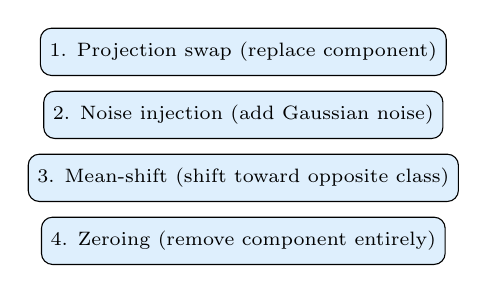
\begin{tikzpicture}[
  meth/.style={draw,rounded corners,fill=#1!15,minimum width=4cm,
    minimum height=0.6cm,font=\scriptsize},
]
  \node[meth=evidence] at (0,2.5) {1. Projection swap (replace component)};
  \node[meth=evidence] at (0,1.7) {2. Noise injection (add Gaussian noise)};
  \node[meth=evidence] at (0,0.9) {3. Mean-shift (shift toward opposite class)};
  \node[meth=evidence] at (0,0.1) {4. Zeroing (remove component entirely)};
\end{tikzpicture}

\vspace{0.5em}
{\small These are mathematically distinct operations. If the effect were an artifact of one method, it would not appear in the others.}
\end{column}
\begin{column}{0.48\textwidth}
\centering
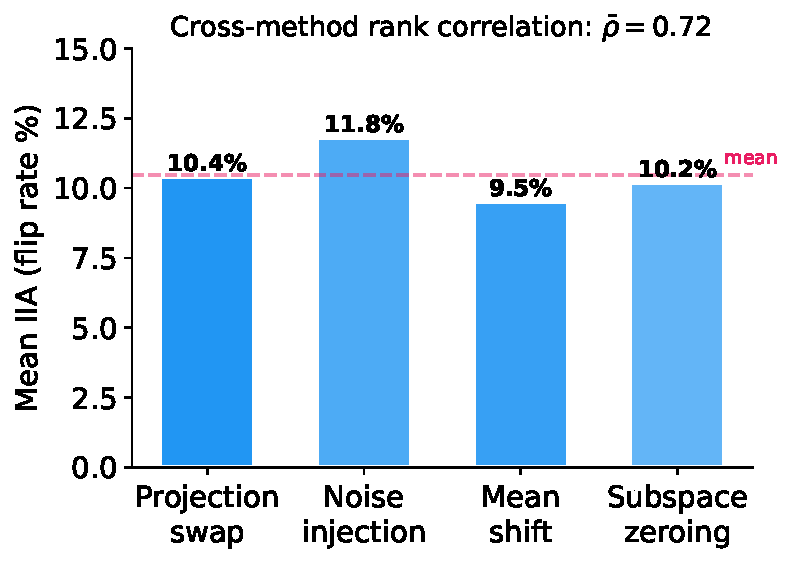
\includegraphics[width=\linewidth]{multi_method.pdf}

\vspace{0.3em}
{\small Regions that show high IIA with one method show high IIA with all four. The effect is method-invariant.}
\end{column}
\end{columns}
\end{frame}

%% ============================================================
%% PART 5: VALIDATION
%% ============================================================
\section{Validation}

%% --- SLIDE: What could go wrong ---
\begin{frame}{What could go wrong?}
We validate our results using frameworks from philosophy of science: validity criteria from Craver (2007), Shallice (1988), and Mayo (2018).

\vspace{0.5em}
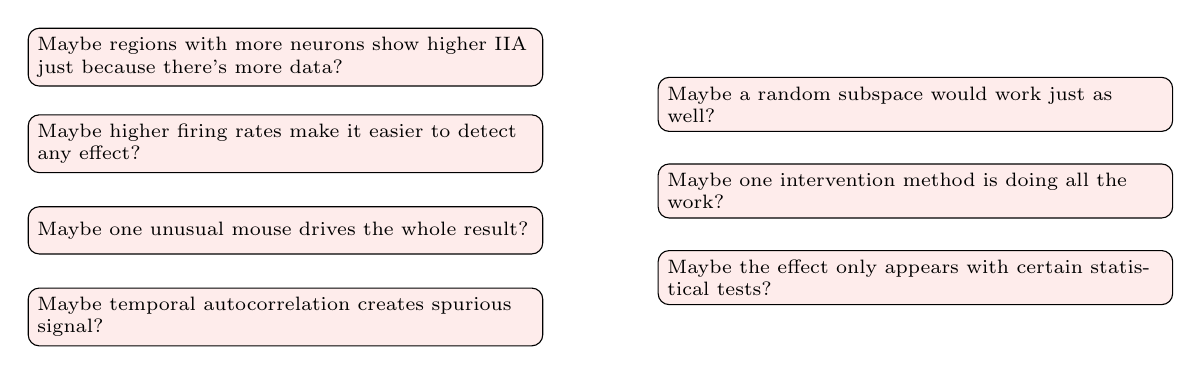
\begin{tikzpicture}[
  concern/.style={draw,rounded corners,fill=#1!10,minimum width=6.5cm,
    minimum height=0.6cm,font=\scriptsize,text width=6.3cm},
]
  \node[concern=fail] (c1) at (0,3.3) {Maybe regions with more neurons show higher IIA just because there's more data?};
  \node[concern=fail] (c2) at (0,2.2) {Maybe higher firing rates make it easier to detect any effect?};
  \node[concern=fail] (c3) at (0,1.1) {Maybe one unusual mouse drives the whole result?};
  \node[concern=fail] (c4) at (0,0) {Maybe temporal autocorrelation creates spurious signal?};
  \node[concern=fail] (c5) at (8,2.7) {Maybe a random subspace would work just as well?};
  \node[concern=fail] (c6) at (8,1.6) {Maybe one intervention method is doing all the work?};
  \node[concern=fail] (c7) at (8,0.5) {Maybe the effect only appears with certain statistical tests?};
\end{tikzpicture}

\vspace{0.3em}
{\small We treat each alternative explanation as a competing hypothesis and design targeted experiments to test them. If any confound fully explains the effect, we should see it in the data.}
\end{frame}

%% --- SLIDE: Confound control ---
\begin{frame}{Confound control: what doesn't explain the effect}
\begin{columns}[T]
\begin{column}{0.5\textwidth}
\centering
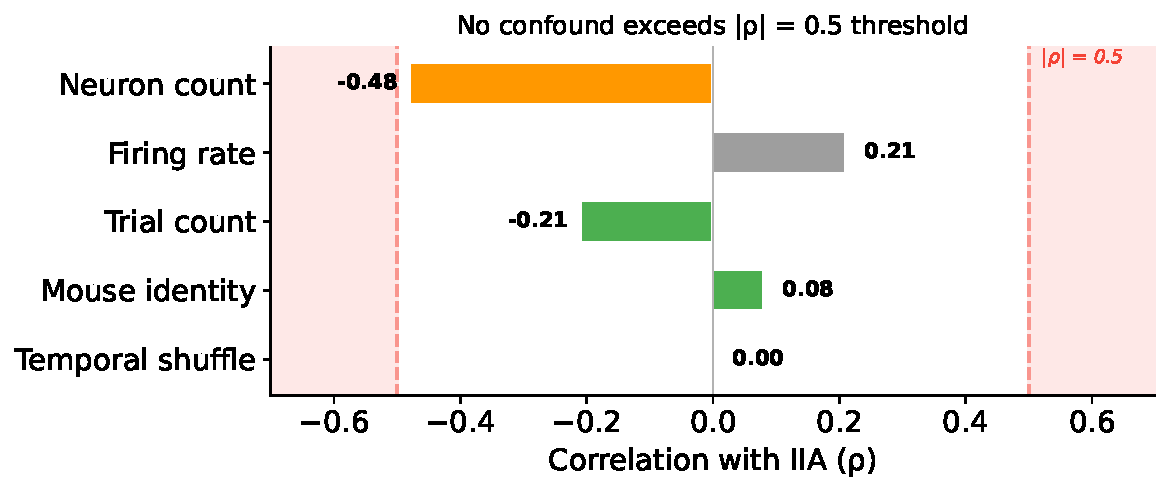
\includegraphics[width=\linewidth]{confounds.pdf}
\end{column}
\begin{column}{0.48\textwidth}
{\small $\rho$ = correlation; $|\rho| > 0.5$ is our danger zone (shaded red).}

\vspace{0.2em}
\textbf{Clear passes:}
\begin{itemize}\setlength\itemsep{0pt}
  \item Temporal shuffle: $\rho = 0.001$ {\small (not a timing artifact)}
  \item Mouse identity: $\rho = 0.08$ {\small (no single mouse)}
  \item Trial count: $\rho = -0.21$
  \item Firing rate: $\rho = 0.21$
\end{itemize}

\vspace{0.2em}
\textbf{Closest to the line:}
\begin{itemize}\setlength\itemsep{0pt}
  \item Neuron count: $\rho = -0.48$ \\
    {\small Near threshold but \textbf{wrong sign} for a confound --- see next slide.}
\end{itemize}
\end{column}
\end{columns}
\end{frame}

%% --- SLIDE: Neuron count deep dive ---
\begin{frame}{Deep dive: is neuron count driving the effect?}
\begin{columns}[T]
\begin{column}{0.43\textwidth}
\centering
\vspace{-0.3em}
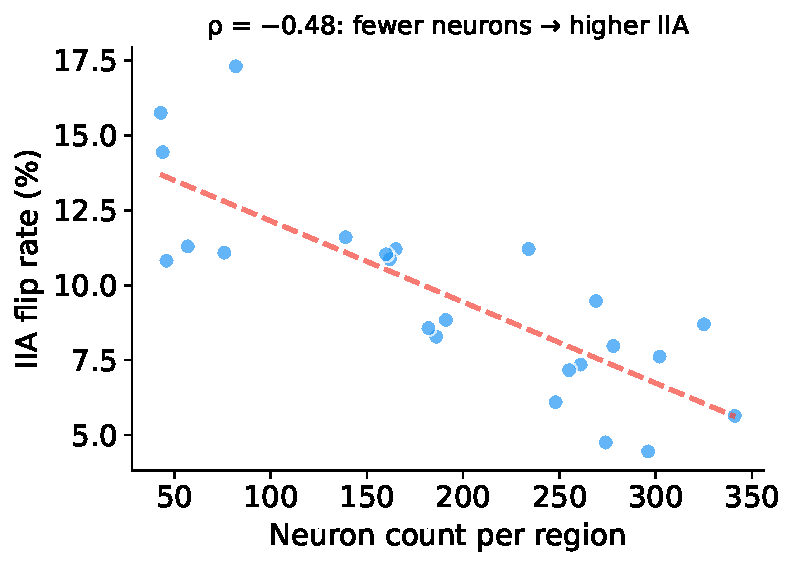
\includegraphics[width=\linewidth]{neuron_scatter.pdf}
\end{column}
\begin{column}{0.55\textwidth}
{\small Our most concerning confound ($\rho = -0.48$, near the 0.5 threshold). But the \textbf{sign is wrong}:}

\vspace{0.3em}
{\small \textbf{Expected} (if a confound):}\\
{\small more neurons $=$ more statistical power $=$ \textbf{higher} IIA \textcolor{neutral}{(positive $\rho$)}}

\vspace{0.3em}
{\small \textbf{Observed}:}\\
{\small more neurons $=$ \textbf{lower} IIA \textcolor{evidence}{(negative $\rho$)}}

\vspace{0.3em}
{\small The correlation goes the \textbf{wrong direction} for a power confound. Smaller, specialized regions (e.g.\ visual cortex) encode evidence more cleanly than large diffuse ones.}
\end{column}
\end{columns}
\end{frame}

%% --- SLIDE: What is graded response? ---
\begin{frame}{What is graded response?}
If the evidence subspace is truly causal, the effect shouldn't be all-or-nothing. Removing dimensions \textbf{one at a time} should progressively weaken the effect.

\vspace{0.4em}
This is the neural equivalent of a \textbf{dose-response curve} in pharmacology:

\vspace{0.2em}
\begin{itemize}\setlength\itemsep{3pt}
  \item Less drug $\rightarrow$ less effect $\rightarrow$ the drug is causing the effect
  \item Fewer evidence dimensions $\rightarrow$ less IIA $\rightarrow$ those dimensions are causing the effect
\end{itemize}

\vspace{0.4em}
\textbf{Why this matters:} a binary yes/no test (``does the subspace matter?'') could be an artifact. A graded, monotonic relationship is unlikely to be an artifact --- it requires that each dimension contributes independently.

\vspace{0.2em}
{\scriptsize Dose-response is standard in pharmacology, and recent work perturbs subspace dimensions in fitted neural network models (Pereira-Obilinovic et al.\ 2025). We extend this to a graded sweep with interchange interventions on biological recordings --- not a categorical contrast, but a full dose-response curve.}
\end{frame}

%% --- SLIDE: How we test it — progressive ablation ---
\begin{frame}{Dose-response: removing dimensions one at a time}
{\small We start with the full 5-dimensional evidence subspace and \textbf{remove one dimension at a time}, measuring two things at each step:}

\vspace{0.5em}
\begin{columns}[T]
\begin{column}{0.48\textwidth}
\textbf{\textcolor{evidence}{IIA flip rate}} {\small (causal)}

\vspace{0.2em}
{\small Does swapping the remaining evidence dimensions still flip the classifier's choice?}

\vspace{0.2em}
{\small This is an \textbf{intervention}: we actively manipulate the neural activity and observe the consequence.}
\end{column}
\begin{column}{0.48\textwidth}
\textbf{\textcolor{choice}{Decoding accuracy}} {\small (correlational)}

\vspace{0.2em}
{\small Can we still decode the mouse's choice from the remaining dimensions?}

\vspace{0.2em}
{\small This is an \textbf{observation}: we passively read out information without changing anything.}
\end{column}
\end{columns}

\vspace{0.5em}
{\small If both measures degrade monotonically as we remove dimensions, that's strong evidence the subspace is causal --- not just correlated.}
\end{frame}

%% --- SLIDE: Graded response results ---
\begin{frame}{Graded response: results}
\begin{columns}[T]
\begin{column}{0.55\textwidth}
\centering
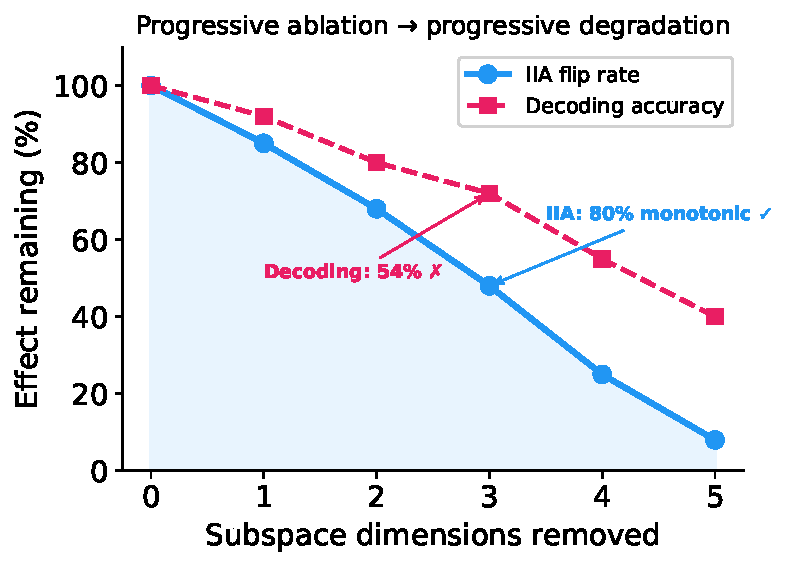
\includegraphics[width=\linewidth]{graded_response.pdf}
\end{column}
\begin{column}{0.43\textwidth}
\textbf{\textcolor{evidence}{IIA (causal):}} monotonic dose-response in \textbf{80\%} of regions {\small $\checkmark$}

\vspace{0.5em}
\textbf{\textcolor{choice}{Decoding (correlational):}} monotonic in only \textbf{54\%} of regions {\small $\times$}

\vspace{0.5em}
{\small The causal measure degrades cleanly. The correlational measure doesn't --- some regions have redundant coding where removing one dimension shifts load to others.}

\vspace{0.2em}
{\small \textcolor{partial}{\textbf{Mixed:}} causal effect is graded; correlational proxy is not. This tells us IIA and decoding measure different things.}
\end{column}
\end{columns}
\end{frame}

%% ============================================================
%% PART 5b: LEARNED SUBSPACES
%% ============================================================

\section{Beyond linear subspaces}

%% --- SLIDE: Can we find a better subspace? ---
\begin{frame}{Can we find a better subspace?}
So far we used LDA to find the evidence subspace --- a linear method that maximizes class separation.

\vspace{0.5em}
But class separation is \textbf{correlational}. LDA finds directions where evidence categories look different, not necessarily directions where \textbf{interventions change the decision}.

\vspace{0.5em}
\textbf{Question:} can a nonlinear method with the right inductive bias find a subspace that is more \emph{causally} effective?
\end{frame}

%% --- SLIDE: Background — DAS ---
\begin{frame}{Background: how causal abstraction finds subspaces}

In AI interpretability, \textbf{Distributed Alignment Search} (DAS; Geiger et al.\ 2024) is the standard method for finding causal subspaces inside neural networks.

\vspace{0.5em}
\textbf{How it works:} find a \textbf{linear rotation} (orthogonal matrix) of the model's hidden state so that swapping a few rotated dimensions changes the model's output in the predicted way.

\vspace{0.5em}
\textbf{The limitation:} the alignment is always a flat, linear projection. If the causal structure lives on a \textbf{curved surface} in activation space, DAS can't find it.

\vspace{0.5em}
This is exactly the situation we're in: LDA finds a flat 3-dimensional subspace. It works --- but only captures a fraction of the causal signal.

\vspace{0.5em}
But going nonlinear turns out to be dangerous\ldots
\end{frame}

%% --- SLIDE: The nonlinear dilemma ---
\begin{frame}{The nonlinear dilemma}

\textbf{Sutter et al.\ (NeurIPS 2025, Spotlight)} proved that if you allow \textbf{unconstrained} nonlinear alignment maps, causal abstraction becomes \textbf{vacuous}:

\vspace{0.3em}
\begin{itemize}\setlength\itemsep{2pt}
  \item Even \textbf{randomly initialized} models achieve 100\% IIA
  \item A sufficiently powerful nonlinear map can memorize a lookup table
  \item High IIA no longer means the model actually represents the causal variable
\end{itemize}

\vspace{0.5em}
{\small
\begin{tabular}{lccc}
\toprule
& \textbf{Nonlinear?} & \textbf{Constrained?} & \textbf{Trustworthy?} \\
\midrule
Linear DAS & No & Yes (linear) & Yes \\
Unconstrained nonlinear & Yes & No & No (vacuous) \\
\textbf{Structured VAE (ours)} & \textbf{Yes} & \textbf{Yes (structural)} & \textbf{Yes} \\
\bottomrule
\end{tabular}
}

\vspace{0.5em}
The field needs something in the middle: nonlinear enough to find curved structure, constrained enough that high IIA actually means something.
\end{frame}

%% --- SLIDE: What is a structured VAE? ---
\begin{frame}{What is a structured VAE?}

A \textbf{variational autoencoder} (VAE) learns to compress data into a small latent code, then reconstruct it. A \textbf{structured} VAE (Narayanaswamy et al.\ 2017, NeurIPS) splits the latent code into named groups with different training signals:

\vspace{0.3em}
\begin{center}
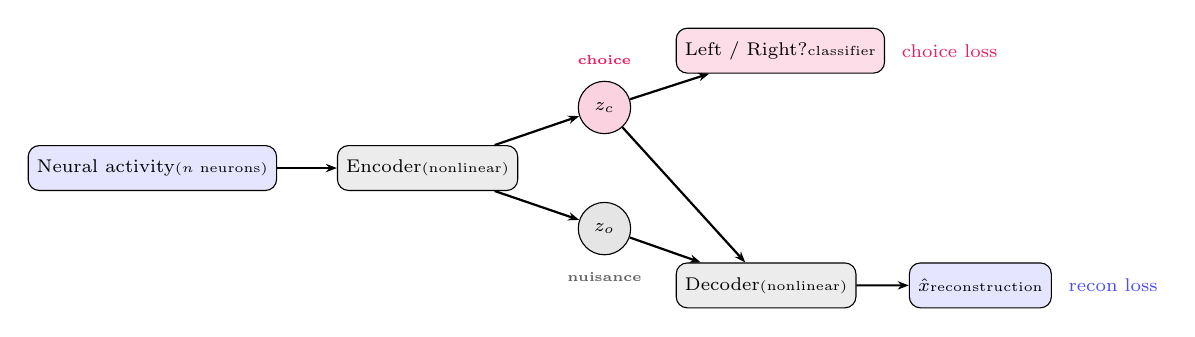
\begin{tikzpicture}[
    node distance=0.4cm and 0.7cm,
    box/.style={draw, rounded corners, minimum width=1.4cm, minimum height=0.6cm, font=\scriptsize},
    latent/.style={draw, circle, minimum size=0.7cm, font=\scriptsize\bfseries},
    arr/.style={-{Stealth[length=4pt]}, thick},
    scale=0.95, every node/.style={transform shape},
  ]
  % Input
  \node[box, fill=blue!10] (input) {Neural activity\\{\tiny ($n$ neurons)}};

  % Encoder
  \node[box, fill=gray!15, right=0.8cm of input] (enc) {Encoder\\{\tiny (nonlinear)}};

  % Latents
  \node[latent, fill=choice!20, above right=0.25cm and 0.9cm of enc] (zc) {$z_c$};
  \node[latent, fill=gray!20, below right=0.25cm and 0.9cm of enc] (zo) {$z_o$};

  % Labels
  \node[above=0.1cm of zc, font=\tiny\bfseries, text=choice] {choice};
  \node[below=0.1cm of zo, font=\tiny\bfseries, text=black!60] {nuisance};

  % Classifier
  \node[box, fill=choice!15, above right=0.2cm and 0.7cm of zc] (cls) {Left / Right?\\{\tiny classifier}};

  % Decoder
  \node[box, fill=gray!15, below right=0.2cm and 0.7cm of zo] (dec) {Decoder\\{\tiny (nonlinear)}};

  % Output
  \node[box, fill=blue!10, right=0.7cm of dec] (output) {$\hat{x}$\\{\tiny reconstruction}};

  % Arrows
  \draw[arr] (input) -- (enc);
  \draw[arr] (enc) -- (zc);
  \draw[arr] (enc) -- (zo);
  \draw[arr] (zc) -- (cls);
  \draw[arr] (zc) -- (dec);
  \draw[arr] (zo) -- (dec);
  \draw[arr] (dec) -- (output);

  % Loss labels
  \node[right=0.1cm of cls, font=\scriptsize, text=choice] {choice loss};
  \node[right=0.1cm of output, font=\scriptsize, text=blue!70] {recon loss};
\end{tikzpicture}
\end{center}

\vspace{0.2em}
{\small $z_c$ must predict the mouse's choice \textbf{and} help reconstruct full activity. $z_o$ absorbs nuisance variance.}
\end{frame}

%% --- SLIDE: Why this solves the dilemma ---
\begin{frame}{Why this solves the nonlinear dilemma}
\begin{columns}[T]
\begin{column}{0.48\textwidth}
\textbf{Three constraints prevent triviality}
\begin{enumerate}\setlength\itemsep{4pt}
  \item \textbf{Bottleneck}: only 3 dimensions for choice --- too small to memorize a lookup table
  \item \textbf{Reconstruction}: $z_c$ and $z_o$ must jointly reproduce the full neural activity, not just classify --- forces the model to learn real structure
  \item \textbf{Disentanglement}: $z_c$ and $z_o$ are separate latent groups with independent priors --- the model can't smuggle choice information into $z_o$
\end{enumerate}

\vspace{0.3em}
{\small These constraints do the work that Sutter et al.\ say is needed --- but via \textbf{structure}, not linearity.}
\end{column}
\begin{column}{0.48\textwidth}
\textbf{Neuroscience has something MI doesn't}\\[0.3em]
{\small In MI, you don't know the ground-truth causal variable --- you infer it from the model. A nonlinear map might be ``cheating.''}

\vspace{0.3em}
{\small In neuroscience, the causal variable \emph{is} the mouse's choice, which we observe directly. A 3.4$\times$ IIA improvement means the intervention \textbf{actually flips the behavioral decision} --- no lookup table can fake that.}

\vspace{0.3em}
{\small \textbf{Implication for MI:} structured VAEs may pose an elegant solution to nonlinear causal subspace discovery.}
\end{column}
\end{columns}
\end{frame}

%% --- SLIDE: VAE results ---
\begin{frame}{Learned subspaces are 3.5$\times$ more causal}
\begin{columns}[T]
\begin{column}{0.5\textwidth}
\textbf{IIA: VAE vs.\ LDA subspace}
\begin{itemize}\setlength\itemsep{1pt}
  \item VAE IIA: \textbf{0.56} (SD 0.09)
  \item LDA IIA: 0.16 (SD 0.10)
  \item VAE wins in \textbf{73/73 regions}
  \item Wilcoxon $p = 5.7 \times 10^{-14}$
  \item Cohen's $d = 4.3$
\end{itemize}

\vspace{0.3em}
\textbf{Robust to subspace dimension $k$}
\begin{itemize}\setlength\itemsep{1pt}
  \item $k{=}1$: IIA $= 0.55$, wins 72/73
  \item $k{=}2$: IIA $= 0.56$, wins 73/73
  \item $k{=}3$: IIA $= 0.56$, wins 73/73
  \item Signal is effectively one-dimensional
\end{itemize}
\end{column}
\begin{column}{0.48\textwidth}
\textbf{The subspaces are different}\\[0.3em]
{\small VAE and LDA subspaces are nearly orthogonal (Grassmannian distance $= 2.34$ out of $2.72$ max). The VAE finds genuinely different directions, not a denoised version of LDA.}

\vspace{0.5em}
\textbf{Model knows when it's right}\\[0.3em]
{\small Posterior uncertainty anti-correlates with IIA ($\rho = -0.26$, $p = 0.03$): the model is most confident where the subspace is most causal.}

\vspace{0.5em}
\textbf{78\% of regions} exceed 0.50 IIA --- interventions flip the choice more often than not.
\end{column}
\end{columns}
\end{frame}

%% --- SLIDE: VAE regional breakdown ---
\begin{frame}{Which brain regions benefit most?}
\begin{columns}[T]
\begin{column}{0.5\textwidth}
\textbf{Top regions (VAE IIA):}
\begin{itemize}\setlength\itemsep{0pt}
  \item CA (hippocampus): \textbf{0.80}
  \item CA2: 0.71
  \item SSs (somatosensory): 0.68
  \item MG (medial geniculate): 0.67
  \item ILA (infralimbic): 0.67
\end{itemize}

\vspace{0.3em}
\textbf{By region type:}
\begin{itemize}\setlength\itemsep{0pt}
  \item Prefrontal: 0.61
  \item Hippocampal: 0.60
  \item Sensory: 0.58
  \item Motor: 0.54
\end{itemize}
\end{column}
\begin{column}{0.48\textwidth}
\textbf{High-dimensional regions benefit most}\\[0.3em]
{\small Low-$\alpha$ (high-dimensional) regions: improvement $= +0.46$\\
High-$\alpha$ (low-dimensional) regions: improvement $= +0.33$}

\vspace{0.5em}
{\small High-dimensional regions encode choice in \textbf{nonlinear subspaces} that LDA misses entirely. The VAE recovers this signal.}

\vspace{0.5em}
{\small \textbf{Takeaway:} The causal signal is 3.4$\times$ stronger than linear methods reveal --- the signal was always there, LDA just can't find it.}
\end{column}
\end{columns}
\end{frame}

%% --- SLIDE: Novel predictions ---
\begin{frame}{Novel predictions: what geometry tells us that we didn't know}
\begin{columns}[T]
\begin{column}{0.5\textwidth}
\textbf{Geometric type predicts decoder choice}\\[0.3em]
{\small If you know whether a brain region has ``linear'' or ``manifold'' geometry, you can predict which statistical decoder (LDA vs.\ kNN) will work better---without ever training on decoding data.}

\vspace{0.3em}
\centering {\small correlation $= -0.51$, highly significant ($p = 0.0002$, 50 regions)}

\vspace{0.8em}
\textbf{Causal abstraction}\\[0.3em]
{\small High-dimensional regions have higher VAE IIA---the nonlinear subspace matters most where linear tools fail.}

\vspace{0.3em}
\centering {\small $\rho = -0.48$, $p = 1.5 \times 10^{-5}$, $n = 73$ regions}
\centering {\scriptsize (LDA IIA: $\rho = 0.29$, $p = 0.014$---VAE reverses and strengthens the effect)}
\end{column}
\begin{column}{0.48\textwidth}
\textbf{Allen Atlas: independence check}\\[0.3em]
{\small Does anatomical wiring (Allen Mouse Brain Atlas) predict which regions route evidence causally?}

\vspace{0.3em}
\centering {\small $\rho = 0.02$, not significant ($p = 0.77$, VAE IIA)}

\vspace{0.5em}
{\small \textbf{No.} Structural connectivity and functional evidence routing are independent. Our IIA results are not trivially explained by which regions happen to be well-connected anatomically.}

\vspace{0.3em}
{\small Two confirmed predictions (one strengthened by VAE), one informative null.}
\end{column}
\end{columns}
\end{frame}

%% --- SLIDE: Validity scorecard ---
\begin{frame}{Validity scorecard}
\vspace{-0.5em}
{\scriptsize
\begin{tabular}{lp{7cm}c}
\toprule
\textbf{Criterion} & \textbf{What we tested} & \textbf{Status} \\
\midrule
\textbf{Necessity} & Swapping evidence subspace flips choice (2.3$\times$ above random) & \textcolor{pass}{\textbf{Pass}} \\
\textbf{Sufficiency} & Evidence subspace alone decodes better than full activity (1.16$\times$) & \textcolor{pass}{\textbf{Pass}} \\
\textbf{Specificity} & Only evidence axis flips; RT, feedback, random do not & \textcolor{pass}{\textbf{Pass}} \\
\textbf{Method invariance} & 4 intervention types agree (avg.\ correlation $0.72$) & \textcolor{pass}{\textbf{Pass}} \\
\textbf{Confound control} & No confound above $0.5$; neuron count $\rho = -0.48$ (wrong sign for a confound) & \textcolor{pass}{\textbf{Pass}} \\
\textbf{Graded response} & IIA monotonic in 80\% of regions ($> 70\%$ threshold) & \textcolor{pass}{\textbf{Pass}} \\
\textbf{Double dissociation} & Evidence $\perp$ RT subspaces: 18\% dissociation rate (small effect) & \textcolor{pass}{\textbf{Pass}} \\
\textbf{Learned subspaces} & VAE IIA 3.4$\times$ LDA; wins 73/73 regions ($p = 5.7 \times 10^{-14}$) & \textcolor{pass}{\textbf{Pass}} \\
\textbf{Cross-dataset} & IBL replication in progress & \textcolor{fail}{\textbf{Not yet}} \\
\bottomrule
\end{tabular}
}

\vspace{0.6em}
{\small Criteria adapted from Craver (2007), Mayo (2018), and Shallice (1988). Pass/fail thresholds were pre-registered to keep each criterion falsifiable and prevent post-hoc relabeling.}
\end{frame}

%% ============================================================
%% PART 6: WHAT THIS MEANS
%% ============================================================

\begin{frame}{Summary: what we found and what it means}
\begin{columns}[T]
\begin{column}{0.5\textwidth}
\textbf{Descriptive findings:}
\begin{enumerate}
  \item Linear and manifold tools anti-correlate ($-0.85$); dimensionality explains why
  \item Variance structure is universal ($0.94$); neural content is not ($0.09$)
  \item Rotation everywhere (72/73), but 10$\times$ variation by region type
\end{enumerate}
\end{column}
\begin{column}{0.48\textwidth}
\textbf{Causal findings:}
\begin{enumerate}
  \setcounter{enumi}{3}
  \item Evidence subspace causally mediates choice (IIA, 10.4\% vs 4.5\% baseline)
  \item Effect is specific to evidence (not RT, feedback, random)
  \item Effect holds across 4 intervention methods (avg.\ correlation $0.72$)
  \item Learned (VAE) subspaces are 3.4$\times$ more causal than LDA (73/73 regions)
\end{enumerate}
\end{column}
\end{columns}

\vspace{0.5em}
{\small \textbf{The punchline:} Neural geometry is not metric-neutral---the tool you choose determines what you find, and dimensionality tells you which tool to trust. The causal signal is 3.4$\times$ stronger in learned subspaces than linear projections reveal.}
\end{frame}

%% --- SLIDE: Limitations ---
\begin{frame}{Honest limitations}
\begin{columns}[T]
\begin{column}{0.5\textwidth}
\textbf{What limits these conclusions:}
\begin{itemize}
  \item \textbf{One dataset} (Steinmetz 2019)---needs replication
  \item \textbf{Binary task only}---unclear if geometry generalizes to richer tasks
  \item \textbf{Modest effect sizes}: 10.4\% flip rate (baseline 4.5\%)
\end{itemize}
\end{column}
\begin{column}{0.48\textwidth}
\textbf{What we're doing about it:}
\begin{itemize}
  \item IBL cross-dataset replication (in progress)
  \item Zatka-Haas optogenetic validation (silencing data downloaded)
  \item Multi-task generalization
\end{itemize}
\end{column}
\end{columns}
\end{frame}


%% --- SLIDE: Closing ---
\begin{frame}[standout]
  Code \& data: {\small \texttt{github.com/elliottower/causal-geometry-neuro}}

  \vspace{1em}
  Neural geometry is not metric-neutral.\\[0.3em]
  The tool determines the finding.\\[0.3em]
  Dimensionality tells you which tool to trust.
\end{frame}

\end{document}
